%% ceci est un commentaire 
%% il faut toujours commencer par \documentclass[type de papier, taille de texte]{sytle du document}
\documentclass[a4paper,10pt]{report} %%%% sytle du document : report/book/article


%%%%%%%%%%%%%%%%%%%%%%%%%%%%%%%%%%%%%%%%%%%%%%%%%%%%%%%%%%%%%%%%%%%%%%%%%%%%%%%
%% la suite est une collection des "package" ou des "librararies" pour utiliser des codes spécifiques

%% il vous suffit de les copie-coller quand vous créez un nouveau document TeX (ou bien en ajouter plus si besoin).
\usepackage[utf8]{inputenc} %% pour les accents en français
\usepackage[frenchb]{babel} %% pour un format français
\usepackage{graphicx} %% pour afficher des graphiques
\usepackage{amsmath} %% pour écrire des symboles (maths), des équations, etc.
\usepackage{amssymb}
\usepackage{color}
\usepackage{bm} %% pour lister des citations/la biblio
\usepackage{hyperref} %% pour inserer des liens internet
\usepackage{cleveref} %% pour faire des références uax équations, tableaux, etc.
\usepackage{cite}
\usepackage{float}
%\usepackage{setspace} %% pour changer l'espace entre les lignes
%\linespread{1.6} %% pour changer l'espace entre les lignes



%%%%%%%%%%%%%%%%%%%%%%%%%%%%%%%%%%%%%%%%%%%%%%%%%
% Default fixed font does not support bold face
\DeclareFixedFont{\ttb}{T1}{txtt}{bx}{n}{8} % for bold
\DeclareFixedFont{\ttm}{T1}{txtt}{m}{n}{8}  % for normal

% Custom colors
\usepackage{color}
\definecolor{deepblue}{rgb}{0,0,0.5}
\definecolor{deepred}{rgb}{0.6,0,0}
\definecolor{deepgreen}{rgb}{0,0.5,0}

\usepackage{listings}

% Python style for highlighting
\newcommand\pythonstyle{\lstset{
language=Python,
breaklines=true,
basicstyle=\ttm,
otherkeywords={self},             % Add keywords here
keywordstyle=\ttb\color{deepblue},
emph={MyClass,__init__},          % Custom highlighting
emphstyle=\ttb\color{deepred},    % Custom highlighting style
stringstyle=\color{deepgreen},
frame=tb,                         % Any extra options here
showstringspaces=false 
           % 
}}


% Python environment
\lstnewenvironment{python}[1][]
{
\pythonstyle
\lstset{#1}
}
{}

% Python for external files
\newcommand\pythonexternal[2][]{{
\pythonstyle
\lstinputlisting[#1]{#2}}}

% Python for inline
\newcommand\pythoninline[1]{{\pythonstyle\lstinline!#1!}}


%%%%%%%%%%%%%%%%%%%%%%%%%%%%%%%%%%%%%%%%%%%%%%%%%%%%%%%%%%%%%%%%%%%%%%%%%%%%%%%
\title{\textbf{Vibrations d'une Disque}} %% choissez un titre approprié à votre sujet
\author{par\\MAAMIR Mohamed\\ZHANG Xunjie\\MOHAMED Muhammad\\GOETZ Kim\\pour le DM de l'UE Introduction aux vibrations des structures M1} %% utilisez \\ pour une nouvelle ligne
\date{fait le 08 janvier 2017} %% pour afficher la date actuelle commenter cette ligne














%%%%%%%%%%%%%%%%%%%%%%%%%%%%%%%%%%%%%%%%%%%%%%%%%%%%%%%%%%%%%%%%%%%%%%%%%%%%%%%
%% TOUT ce qui va dans votre rapport doit être entre \begin{document} & \end{document}
\begin{document}
\selectlanguage{french} %% format français
\maketitle %% pour afficher le titre
\tableofcontents %% pour afficher/compiler le sommaire automatiquement
\listoffigures %% pour lister les figures












%%%%%%%%%%%%%%%%%%%%%%%%%%%%%%%%%%%%%%%%%%%%%%%%%%%%%%%%%%%%%%%%%%%%%%%%%%%%%%%
\chapter{Introduction} %% pour commencer un chapitre

Nous allons étudier dans ce DM un système en vibrations forcées amorties. Dans une première partie théorique nous allons modéliser le système à 2 puis N degrés de liberté, dresser les équations du mouvement et calculer la réponse en vibrations forcées. \\ Dans la seconde partie, nous traitons le problème de manière numérique sous Scilab. Analyse modale pour différents degrés de liberté et calcul de la réponse en vibrations forcées en fonction de $\omega$.


\begin{figure}[H]
\begin{center}
	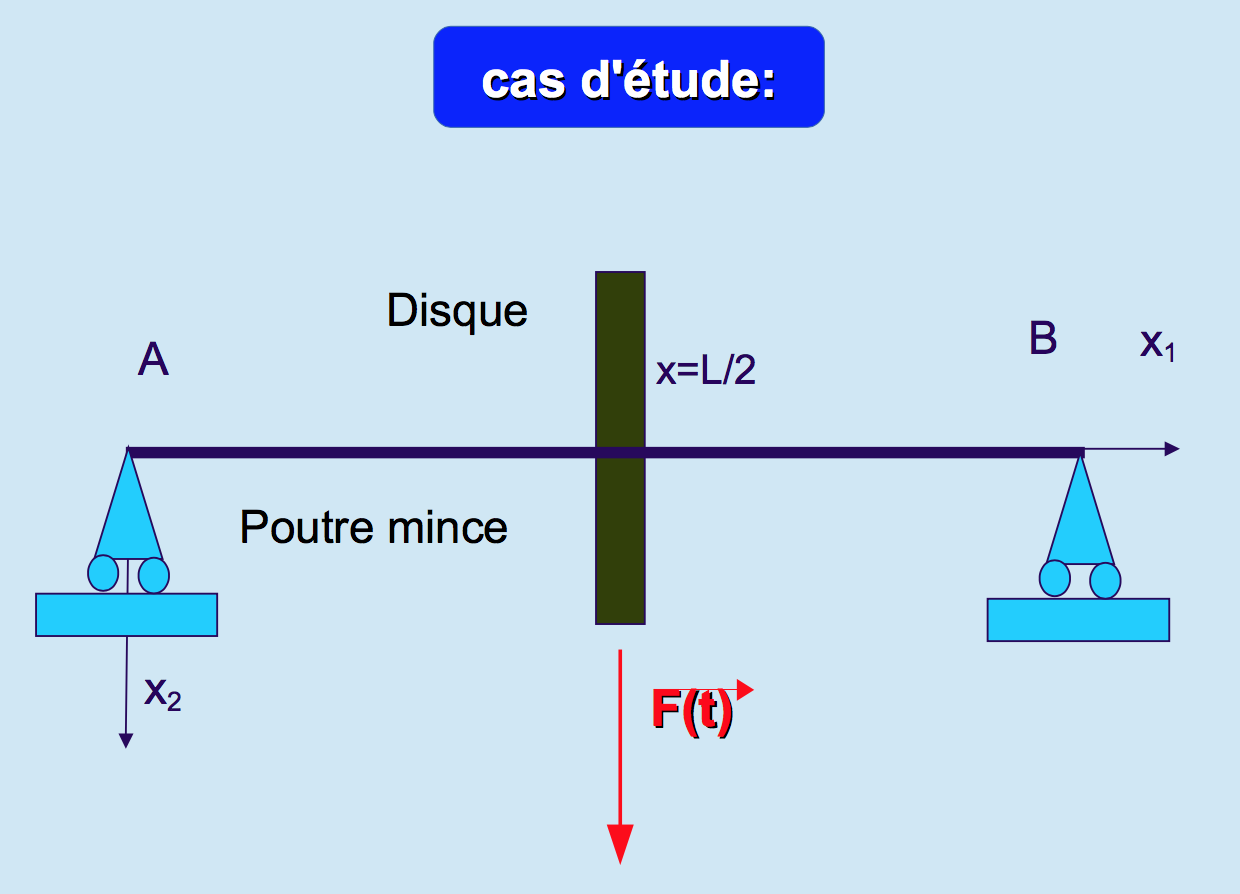
\includegraphics[width=1\textwidth]{sujet.png} 
\end{center} 
\caption{Cas d'étude.}
\end{figure}




\chapter{Théorie}











\begin{figure}[H]
\begin{center}
	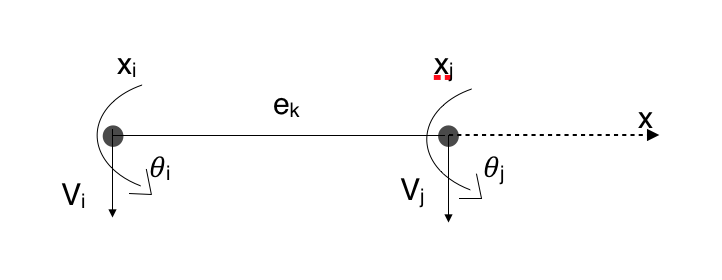
\includegraphics[width=1\textwidth]{schemaelementk.png} 
\end{center} 
\caption{Cas d'étude.}
\end{figure}



On pose que le déplacement est en expression suivante :
\begin{equation}
v(x)=a_0+a_1\frac{x}{L}+a_2\frac{x^2}{L^2}+a_3\frac{x^3}{L^3} \ ,\  \Omega=[x_i,x_j]
\end{equation}


et rotation :
\begin{equation}
\theta(x)=a_1\frac{1}{L}+a_2\frac{2x}{L^2}+a_3\frac{3x^2}{L^3} \ ,\  \Omega=[x_i,x_j]
\end{equation}

On a déplacement et rotation sur $0$ et $\frac{L}{2}$ , ceque on note $v_i$ , $\theta_i$ , $v_j$ , $\theta_j$ \\
\begin{itemize}
    \item[$\bullet$]$v_i$ est déplacement d'une extrémité à $x$=$x_i$ qui est toujour nulle .
    \item[$\bullet$]$\theta_i$ est la rotation d'une extrémité à $x$=$x_i$
    \item[$\bullet$]$v_j$ est déplacement d'autre extrémité à $x$=$x_j$ .
    \item[$\bullet$]$\theta_j$ est la rotation d'autre extrémité à $x$=$x_j$
\end{itemize}


Il y a 4 conditions  , donc on peut camculer la expression de $v(x)$:
\[ 
\left[ \begin{array}{c}v_i\\\\\theta_i\\\\v_j\\\\\theta_j\end{array} \right]
=\left[ \begin{array}{cccc}
1 & 0 & 0 & 0  \\\\
0 & \frac{1}{L} & 0 & 0 \\\\
1 & 1 &1 &1 \\\\
0 & \frac{1}{L} &\frac{2}{L} &\frac{3}{L} 
\end{array} \right]
\left[ \begin{array}{c}a_0\\\\a_1\\\\a_2\\\\a_3\end{array} \right]
\]

Ensuite , on trouver le relation suivante :
\[ 
\left[ \begin{array}{c}a_0\\\\a_1\\\\a_2\\\\a_3\end{array} \right]
=\left[ \begin{array}{cccc}
1 & 0 & 0 & 0  \\\\
0 & L & 0 & 0 \\\\
-3 & -2L &3 &-L \\\\
2 & L & -2 &L
\end{array} \right]
\left[ \begin{array}{c}v_i\\\\\theta_i\\\\v_j\\\\\theta_j\end{array} \right]
\]

et on reprend $v(x)$:

\begin{equation}
v(x)=v_j+L\theta_i\frac{x}{L}+(-3v_i-2L\theta_i+3v_j-L\theta_j)\frac{x^2}{L^2}+(2v_i+L\theta_i-2v_j+L\theta_j)\frac{x^3}{L^3}
\end{equation}

On noté $\xi=\frac{x}{L}$:
\begin{center}
$$v(x)=v_i+L\theta_i\xi+(-3v_i-2L\theta_i+3v_j-L\theta_j)\xi^2+(2v_i+L\theta_i-2v_j+L\theta_j)\xi^3 $$\\
$$v(x)=(1-3\xi^2+2\xi^3)v_i+(\xi-2\xi^2+\xi^3)L\theta_i+(3\xi^2-2\xi^3)v_j+(-\xi^2+\xi^3)L\theta_j$$\\
\end{center}


on noté :
\begin{center}
$\phi_i=1-3\xi^2+2\xi^3$\\$\phi_j=3\xi^2-2\xi^3)$\\$\psi_i=(\xi-2\xi^2+\xi^3)L$\\$\psi_j=(-\xi^2+\xi^3)L$\\
$$v(x)=\phi_iv_i+\phi_j\theta_i+\psi_iv_j+\psi_j\theta_j$$
\end{center}

On cherche la matrice de la masse  par $v(x)$ :
\begin{center}
$$E_c=\frac{1}{2}\int_{x_i}^{x_j}\rho S\dot{v}^2dx=\frac{1}{2}\int_{x_i}^{x_j}\rho S\dot{v}^2\frac{dx}{L}$$\\
$$E_c=\frac{1}{2}\int_{x_i}^{x_j}\rho S(\phi_i\dot{v_i}+\phi_j\dot{\theta_i}+\psi_i\dot{v_j}+\psi_j\dot{\theta_j})^2d\xi$$
\end{center}

Après les calcules on trouve la matrice $\widehat{M}$ :
\[ \widehat{M}=\rho S\int_{x_i}^{x_j}\left[ \begin{array}{cccc}
\phi_i^2 &\phi_i\psi_i& \phi_i\phi_j&\phi_i\psi_j     \\\\
\psi_i\phi_i & \psi_i^2& \psi_i\phi_j&\psi_i\psi_j \\\\
\phi_j\phi_i &\phi_j\psi_i& \phi_j^2&\phi_j\psi_j     \\\\
\psi_j\phi_i &\psi_j\psi_i&\psi_j \phi_j&\psi_j^2    \\\\
 \end{array} \right]dx\]


Nous allons diviser l'étude de notre système en 2 parties : l'étude des modes symétriques et l'étude des modes antisymétriques, associées à 2 modèles spécifiques.
\section{modes antisymétriques}

\begin{figure}[H]
\begin{center}
	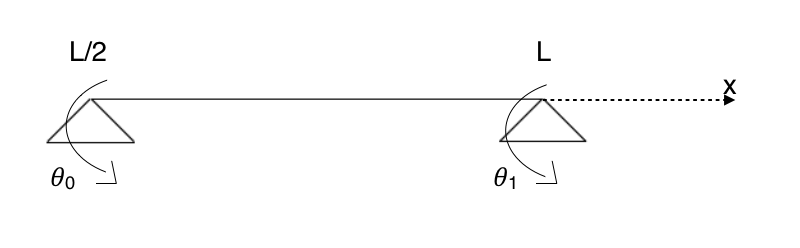
\includegraphics[width=1\textwidth]{schemamodeantisym.png} 
\end{center} 
\caption{Modèle utilisé pour déterminer les modes antisymétriques de notre cas d'étude.}
\end{figure}

\subsection{2 DDL}
\subsubsection{méthode des matrices}

L'équation du mouvement est de la forme générale :
$$ \Bigg[
- \omega^2 \rho S \begin{pmatrix}
   M_{11} & M_{12} \\
   M_{21} & M_{22} 
\end{pmatrix}
+ i \omega \begin{pmatrix}
	\lambda_{11} & \lambda_{12} \\
	\lambda_{21} & \lambda_{22}
\end{pmatrix}
+ \begin{pmatrix}
	K_{11} & K_{12} \\
	K_{12} & K_{22}
\end{pmatrix} \Bigg]
\begin{pmatrix}
	X_{10} \\
	X_{20}
\end{pmatrix}
= \begin{pmatrix}
	0 \\
	F
\end{pmatrix}
$$


\subsection{N DDL}


\begin{figure}[H]
\begin{center}
	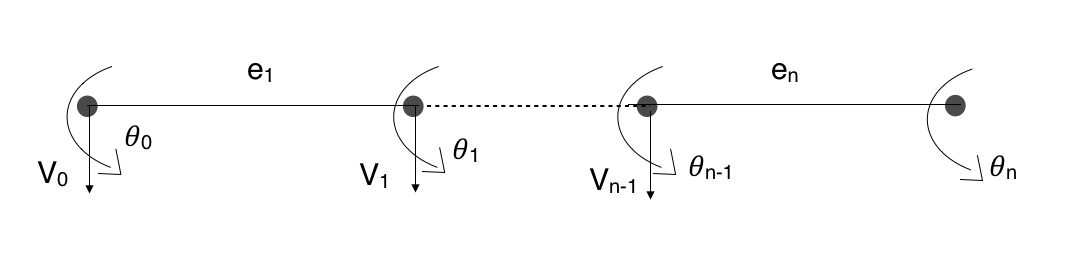
\includegraphics[width=1\textwidth]{casVn.png} 
\end{center} 
\caption{Modèle utilisé pour déterminer les modes antisymétriques de notre cas d'étude.}
\end{figure}


\subsubsection{ matrice élémentaire de masse}
On cherche la matrice de la masse  par $v(x)$ :
\begin{center}
$$E_c=\frac{1}{2}\int_{x_i}^{x_j}\rho S\dot{v}^2dx=\frac{1}{2}\int_{x_i}^{x_j}\rho S\dot{v}^2\frac{dx}{L}$$\\
$$E_c=\frac{1}{2}\int_{x_i}^{x_j}\rho S(\phi_i\dot{v_i}+\phi_j\dot{\theta_i}+\psi_i\dot{v_j}+\psi_j\dot{\theta_j})^2d\xi$$
\end{center}

Après les calcules on trouve la matrice $\widehat{M}$ :
\[ \widehat{M}=\rho S\int_{x_i}^{x_j}\left[ \begin{array}{cccc}
\phi_i^2 &\phi_i\psi_i& \phi_i\phi_j&\phi_i\psi_j     \\\\
\psi_i\phi_i & \psi_i^2& \psi_i\phi_j&\psi_i\psi_j \\\\
\phi_j\phi_i &\phi_j\psi_i& \phi_j^2&\phi_j\psi_j     \\\\
\psi_j\phi_i &\psi_j\psi_i&\psi_j \phi_j&\psi_j^2    \\\\
 \end{array} \right]dx\]
 
 
 \[ \widehat{M_1}=\rho S\int_{x_i}^{x_j}\left[ \begin{array}{cccc}
0 &0&0&0    \\\\
0 & \psi_i^2& \psi_i\phi_j&\psi_i\psi_j \\\\
0&\phi_j\psi_i& \phi_j^2&\phi_j\psi_j     \\\\
0 &\psi_j\psi_i&\psi_j \phi_j&\psi_j^2    \\\\
 \end{array} \right]dx
 \,\,\,\,
 \widehat{M_n}=\rho S\int_{x_i}^{x_j}\left[ \begin{array}{cccc}
\phi_i^2 &\phi_i\psi_i&0&\phi_i\psi_j     \\\\
\psi_i\phi_i & \psi_i^2&0&\psi_i\psi_j \\\\
0 &0& 0&0   \\\\
\psi_j\phi_i &\psi_j\psi_i&0&\psi_j^2 \\\\
 \end{array} \right]dx\]
 
 \subsubsection{matrice élémentaire de raideur}
\[ \widehat{K_{ij}}=\left[ \begin{array}{cccc}
K &0& -K&0     \\\\
0 & K_{\theta}&0&-K_{\theta} \\\\
-K &0& K&0     \\\\
0&-K_{\theta}& 0&K_{\theta}   \\\\
 \end{array} \right]_{v_i \, \theta_i \, v_j \, \theta_j \, } \]
 
 \[ \widehat{K_1}=\left[ \begin{array}{cccc}
0 &0& 0&0     \\\\
0&0&0&-K_{\theta} \\\\
0&0& K&0    \\\\
0&-K_{\theta}&0&0   \\\\
 \end{array} \right]_{v_0 \, \theta_0 \, v_1 \, \theta_1 \, }
 \,\,\,\,
 \widehat{K_n}=\left[ \begin{array}{cccc}
K &0& 0&0     \\\\
0&0&0&-K_{\theta} \\\\
0&0& 0&0    \\\\
0&-K_{\theta}&0&0   \\\\
 \end{array} \right]_{v_{n-1} \, \theta_{n-1} \, v_{n} \, \theta_{n} \, }\]

\subsubsection{matrice élémentaire de amortissement}
\[ \widehat{\lambda_{ij}}=\left[ \begin{array}{cccc}
\lambda &0& -\lambda&0     \\\\
0& \lambda_{\theta}&0&-\lambda_{\theta} \\\\
-\lambda &0& \lambda&0    \\\\
0&-\lambda_{\theta}&0&\lambda_{\theta}    \\\\
 \end{array} \right]_{v_i \, \theta_i \, v_j \, \theta_j \, }\]



\[ \widehat{\lambda_1}=\left[ \begin{array}{cccc}
0 &0& 0&0     \\\\
0&0&0&-\lambda_{\theta} \\\\
0&0& \lambda&0    \\\\
0&-\lambda_{\theta}&0&0   \\\\
 \end{array} \right]_{v_0 \, \theta_0 \, v_1 \, \theta_1 \, }
 \,\,\,\,
  \widehat{\lambda_n}=\left[ \begin{array}{cccc}
\lambda &0& 0&0     \\\\
0&0&0&-\lambda_{\theta} \\\\
0&0& \lambda&0    \\\\
0&-\lambda_{\theta}&0&0   \\\\
 \end{array} \right]_{v_{n-1} \, \theta_{n-1} \, v_{n} \, \theta_{n} \, }\]
 




\section{modes symétriques}


\begin{figure}[H]
\begin{center}
	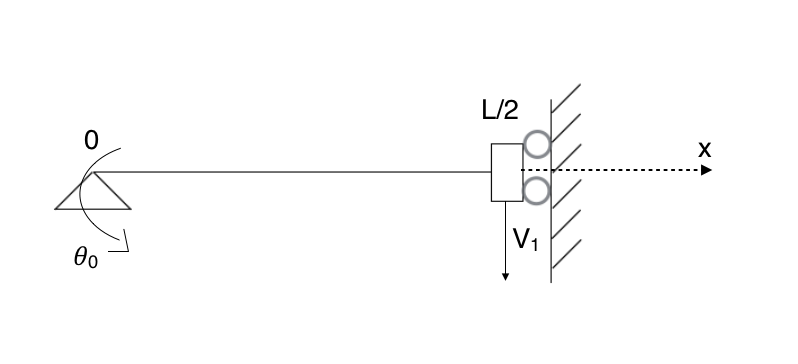
\includegraphics[width=1\textwidth]{SchemaModeSym.png} 
\end{center} 
\caption{Modèle utilisé pour déterminer les modes symétriques.}
\end{figure}

\subsection{2 DDL}
\subsubsection{méthode des matrices}



\subsection{N DDL}

\begin{figure}[H]
\begin{center}
	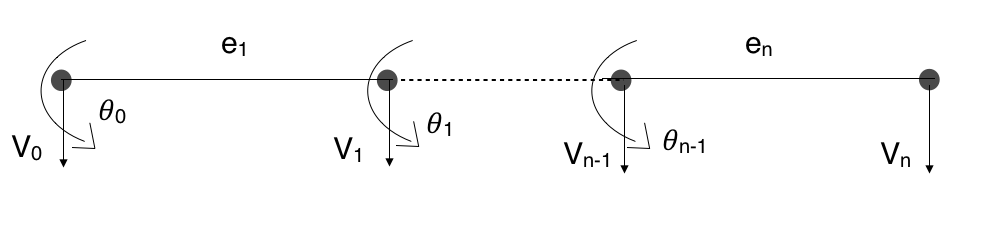
\includegraphics[width=1\textwidth]{CasthetaN.png} 
\end{center} 
\caption{Modèle utilisé pour déterminer les modes antisymétriques de notre cas d'étude.}
\end{figure}



\subsubsection{ matrice élémentaire de masse}
On cherche la matrice de la masse  par $v(x)$ :
\begin{center}
$$E_c=\frac{1}{2}\int_{x_i}^{x_j}\rho S\dot{v}^2dx=\frac{1}{2}\int_{x_i}^{x_j}\rho S\dot{v}^2\frac{dx}{L}$$\\
$$E_c=\frac{1}{2}\int_{x_i}^{x_j}\rho S(\phi_i\dot{v_i}+\phi_j\dot{\theta_i}+\psi_i\dot{v_j}+\psi_j\dot{\theta_j})^2d\xi$$
\end{center}

Après les calcules on trouve la matrice $\widehat{M}$ :
\[ \widehat{M}=\rho S\int_{x_i}^{x_j}\left[ \begin{array}{cccc}
\phi_i^2 &\phi_i\psi_i& \phi_i\phi_j&\phi_i\psi_j     \\\\
\psi_i\phi_i & \psi_i^2& \psi_i\phi_j&\psi_i\psi_j \\\\
\phi_j\phi_i &\phi_j\psi_i& \phi_j^2&\phi_j\psi_j     \\\\
\psi_j\phi_i &\psi_j\psi_i&\psi_j \phi_j&\psi_j^2    \\\\
 \end{array} \right]dx\]
 
 
  \[ \widehat{M_1}=\rho S\int_{x_i}^{x_j}\left[ \begin{array}{cccc}
0 &0&0&0    \\\\
0 & \psi_i^2& \psi_i\phi_j&\psi_i\psi_j \\\\
0&\phi_j\psi_i& \phi_j^2&\phi_j\psi_j     \\\\
0 &\psi_j\psi_i&\psi_j \phi_j&\psi_j^2    \\\\
 \end{array} \right]dx
 \,\,\,\,
 \widehat{M_n}=\rho S\int_{x_i}^{x_j}\left[ \begin{array}{cccc}
\phi_i^2 &\phi_i\psi_i& \phi_i\phi_j&0     \\\\
\psi_i\phi_i & \psi_i^2& \psi_i\phi_j&0 \\\\
\phi_j\phi_i &\phi_j\psi_i& \phi_j^2&0     \\\\
0&0&0&0    \\\\
 \end{array} \right]dx\]
 
 \subsubsection{matrice élémentaire de raideur}
\[ \widehat{K_{ij}}=\left[ \begin{array}{cccc}
K &0& -K&0     \\\\
0 & K_{\theta}&0&-K_{\theta} \\\\
-K &0& K&0     \\\\
0&-K_{\theta}& 0&K_{\theta}   \\\\
 \end{array} \right]_{v_i \, \theta_i \, v_j \, \theta_j \, } \]
 
 \[ \widehat{K_1}=\left[ \begin{array}{cccc}
0 &0& 0&0     \\\\
0&0&0&-K_{\theta} \\\\
0&0& K&0    \\\\
0&-K_{\theta}&0&0   \\\\
 \end{array} \right]_{v_0 \, \theta_0 \, v_1 \, \theta_1 \, }
 \,\,\,\,
 \widehat{K_n}=\left[ \begin{array}{cccc}
K &0& -K&0     \\\\
0&K_{\theta}&0&0 \\\\
-K&0& K&0    \\\\
0&0&0&0   \\\\
 \end{array} \right]_{v_{n-1} \, \theta_{n-1} \, v_{n} \, \theta_{n} \, }\]

\subsubsection{matrice élémentaire de amortissement}
\[ \widehat{\lambda_{ij}}=\left[ \begin{array}{cccc}
\lambda &0& -\lambda&0     \\\\
0& \lambda_{\theta}&0&-\lambda_{\theta} \\\\
-\lambda &0& \lambda&0    \\\\
0&-\lambda_{\theta}&0&\lambda_{\theta}    \\\\
 \end{array} \right]_{v_i \, \theta_i \, v_j \, \theta_j \, }\]



\[ \widehat{\lambda_1}=\left[ \begin{array}{cccc}
0 &0& 0&0     \\\\
0&0&0&-\lambda_{\theta} \\\\
0&0& \lambda&0    \\\\
0&-\lambda_{\theta}&0&0   \\\\
 \end{array} \right]_{v_0 \, \theta_0 \, v_1 \, \theta_1 \, }
 \,\,\,\,
 \widehat{\lambda_n}=\left[ \begin{array}{cccc}
\lambda &0& -\lambda&0     \\\\
0&\lambda_{\theta}&0&0 \\\\
-\lambda&0&\lambda&0    \\\\
0&0&0&0   \\\\
 \end{array} \right]_{v_{n-1} \, \theta_{n-1} \, v_{n} \, \theta_{n} \, }\]
 





\section{équations du mouvement}
\subsection{2 DDL}
L'équation du mouvement est de la forme générale :
$$ \Bigg[
- \omega^2 \rho S \begin{pmatrix}
   M_{11} & M_{12} \\
   M_{21} & M_{22} 
\end{pmatrix}
+ i \omega \begin{pmatrix}
	\lambda_{11} & \lambda_{12} \\
	\lambda_{21} & \lambda_{22}
\end{pmatrix}
+ \begin{pmatrix}
	K_{11} & K_{12} \\
	K_{12} & K_{22}
\end{pmatrix} \Bigg]
\begin{pmatrix}
	X_{10} \\
	X_{20}
\end{pmatrix}
= \begin{pmatrix}
	0 \\
	F
\end{pmatrix}
$$

\subsection{N DDL}
$ \Bigg[
- \omega^2 \rho S \begin{pmatrix}
   M_{11} &\cdots&\cdots&M_{1N} \\
   \vdots & \ddots &&\vdots\\
   \vdots &&\ddots&\vdots\\
   M_{N1}  &\cdots&\cdots&M_{NN}
\end{pmatrix}
+ i \omega \begin{pmatrix}
	\lambda_{11} &\cdots&\cdots&\lambda_{1N} \\
   \vdots & \ddots &&\vdots\\
   \vdots &&\ddots&\vdots\\
   \lambda_{N1}  &\cdots&\cdots&\lambda_{NN}
\end{pmatrix}
+ \begin{pmatrix}
	K_{11} &\cdots&\cdots&K_{1N} \\
   \vdots & \ddots &&\vdots\\
   \vdots &&\ddots&\vdots\\
   K_{N1}  &\cdots&\cdots&K_{NN}
\end{pmatrix} \Bigg]\\
\begin{pmatrix}
	X_{10} \\
	\vdots\\
	\vdots\\
	X_{N0}
\end{pmatrix}
= \begin{pmatrix}
	0 \\
	\vdots\\
	\vdots\\
	F
\end{pmatrix}
$


%%%%%%%%%%%%%%%%%%%%%%%%%%%%%%%%%%
\chapter{Numérique sur SCILAB}









%%%%%%%%%%%%%%%%%%%%%%%%%%%%%%%%%%%%%%%%%%%%%%%%%%%%%%%%%%%%%%%%%%%%%%%%%%%%%%
\chapter{Conclution}


Dans ce DM, nous avons étudié le modèle vibratoire de deux cas de sollicitations sur une même structure. Grâce à une étude statique, nous avons pu établir un modèle vibratoire de la structure et simuler son comportement avec des paramètres physiques et des conditions initiales différentes. Ce modèle a été trouvé en respectant les hypothèses de départ et en s'abstrayant de certains effets comme l'absence de cisaillement au niveau des liaisons, la négligence des masses des poutres verticales ainsi que la négligence de la compression dans le cas 1. N'oublions pas non plus que le bloc a été considéré comme indéformable ce qui ne peut être le cas dans la réalité.

Nous avons pu constater que tant qu'on reste dans le domaine élastique de la structure, la réponse vibratoire dépendait du facteur d'amortissement, de la raideur, de la masse et de la sollicitation initiale. Ainsi, ce sont ces paramètres qu'il faut étudier et modifier si l'on veut changer les propriétés vibratoires de la structure.

Pour conclure, nous pouvons dire que ce DM nous aura permis, en équipe, de mettre en pratique la théorie sur les modèles vibratoire dans le cas des vibrations libres amorties. Cette étude est restée dans un cadre simplifié avec des hypothèses qui reste applicable dans certains cas seulement. Il ne faut jamais perdre de l'oeil les hypothèses de départ qui nous ont permis de construire un modèle. 













%\bibliography{MonBiblio.bib}
%\bibliographystyle{unsrtnat}	
\end{document}
\grid
